% プロコン 2026 展示ポスター A0 2 枚版の 1 枚目（課題とシステム）
% poster.tex（1 枚版）と同じ構成を 2 枚に広げ、文字・図を大きくして情報を足したもの。
% 版面は A1 で組み、poster2_a0.tex が √2 倍して A0 2 ページの poster2_a0.pdf にする。
% ビルド: build_poster.bat をダブルクリック（Tectonic）
\documentclass[24pt,a1paper,portrait,margin=0mm,innermargin=12mm,
  blockverticalspace=5mm,colspace=9mm,subcolspace=8mm]{tikzposter}
% poster2_p1.tex / poster2_p2.tex（A0 2 枚版）で共有する設定。poster.tex（1 枚版）の設定を元に、文字を大きくしたもの
% 寸法・文字サイズは A1 のときの値（poster2_a0.tex で 1.414 倍して A0 にする）
\usepackage{xeCJK}
\setCJKmainfont[BoldFont=HaranoAjiGothic-Bold.otf]{HaranoAjiGothic-Regular.otf}
\setCJKsansfont[BoldFont=HaranoAjiGothic-Bold.otf]{HaranoAjiGothic-Regular.otf}
\setmainfont{texgyreheros-regular.otf}[BoldFont=texgyreheros-bold.otf]
\setsansfont{texgyreheros-regular.otf}[BoldFont=texgyreheros-bold.otf]
\xeCJKsetup{CJKspace=false}

\usepackage{amsmath,amssymb,bm}
\usepackage{enumitem}
\usepackage{graphicx}
\usepackage{array}
\usepackage{fontawesome5}
\usepackage{pgfplots}
\pgfplotsset{compat=1.18}
\usetikzlibrary{positioning,arrows.meta,calc}
\graphicspath{{../../resume/}{../../}}

\setlist{nosep,leftmargin=1.0em,itemsep=4pt}
\renewcommand{\labelitemi}{\textcolor{blue}{\textbullet}}
\setlength{\parindent}{0pt}
\setlength{\parskip}{2pt}

% ---------------------------------------------------------------- 色（DESIGN.md とロゴに合わせる）
\definecolor{navy}{HTML}{164A86}     % ロゴの文字色
\definecolor{blue}{HTML}{0093C4}     % blue-deep
\definecolor{skytint}{HTML}{E3F7FF}
\definecolor{yellow}{HTML}{FFDB4F}
\definecolor{yellowdeep}{HTML}{C99A00}
\definecolor{yellowtint}{HTML}{FFF6DA}
\definecolor{ink}{HTML}{232323}
\definecolor{ink2}{HTML}{5E584C}
\definecolor{paper}{HTML}{F1EFE8}    % ロゴの背景色
\definecolor{card}{HTML}{F6F3EA}
\definecolor{good}{HTML}{1C7A45}
\definecolor{goodtint}{HTML}{E3F4E9}
\definecolor{orange}{HTML}{E2612B}

\definecolorstyle{gemmba}{
  \colorlet{colorOne}{navy}\colorlet{colorTwo}{blue}\colorlet{colorThree}{yellow}
}{
  \colorlet{backgroundcolor}{paper}
  \colorlet{framecolor}{paper}
  \colorlet{titlefgcolor}{navy}
  \colorlet{titlebgcolor}{paper}
  \colorlet{blocktitlebgcolor}{white}
  \colorlet{blocktitlefgcolor}{navy}
  \colorlet{blockbodybgcolor}{white}
  \colorlet{blockbodyfgcolor}{ink}
  \colorlet{innerblocktitlebgcolor}{white}
  \colorlet{innerblocktitlefgcolor}{navy}
  \colorlet{innerblockbodybgcolor}{white}
  \colorlet{innerblockbodyfgcolor}{ink}
  \colorlet{notefgcolor}{ink}
  \colorlet{notebgcolor}{skytint}
  \colorlet{noteframecolor}{blue}
}
\usecolorstyle{gemmba}
\usetitlestyle{Filled}
\usebackgroundstyle{Default}

% ブロック：白いカード。見出しは中央、黄色の下線
\defineblockstyle{gemblock}{
  titlewidthscale=1, bodywidthscale=1, titlecenter,
  titleoffsetx=0pt, titleoffsety=0pt, bodyoffsetx=0mm, bodyoffsety=0mm,
  bodyverticalshift=0mm, roundedcorners=10, linewidth=0pt,
  titleinnersep=3mm, bodyinnersep=6mm
}{
  \ifBlockHasTitle
    \draw[draw=none, fill=white, rounded corners=\blockroundedcorners]
      (blockbody.south west) rectangle (blocktitle.north east);
  \else
    \draw[draw=none, fill=white, rounded corners=\blockroundedcorners]
      (blockbody.south west) rectangle (blockbody.north east);
  \fi
}
\useblockstyle{gemblock}


% ---------------------------------------------------------------- タイトル（2 枚とも同じ帯。右上にページ番号）
% \posttitle{ページの主題}{n/2}
\newcommand{\posttitle}[2]{%
  \settitle{%
    \begin{minipage}[c]{0.36\linewidth}
      
\includegraphics[width=0.95\linewidth]{logo.png}
    \end{minipage}\hfill
    \begin{minipage}[c]{0.62\linewidth}
      \raggedright\color{navy}
      {\fontsize{66pt}{70pt}\selectfont\bfseries 中小企業向けのDX推進システム}\par\vspace{10pt}
      {\fontsize{36pt}{40pt}\selectfont\bfseries\color{blue}#1}\quad
      {\fontsize{26pt}{30pt}\selectfont\bfseries\color{white}\colorbox{navy}{\,#2\,}}\par\vspace{10pt}
      {\fontsize{24pt}{28pt}\selectfont\color{ink2}明石工業高等専門学校\quad 小笠原\,悠太\quad 増永\,惺真\qquad 指導教員：野村\,隼人}
    \end{minipage}}}

% ---------------------------------------------------------------- 部品
% ブロック見出し：文字幅に合わせた黄色の下線
\newcommand{\bt}[1]{\tikz[baseline=(t.base)]{%
  \node[inner sep=0, font=\fontsize{48pt}{54pt}\selectfont\bfseries, text=navy] (t) {#1};
  \fill[yellow] ([xshift=-6mm, yshift=-16pt]t.south west) rectangle ([xshift=6mm, yshift=-6pt]t.south east);}}
\newcommand{\sm}{\fontsize{20pt}{25pt}\selectfont}
\newcommand{\capt}[1]{{\centering\fontsize{20pt}{25pt}\selectfont\color{ink2}#1\par}}
\newcommand{\head}[1]{{\fontsize{32pt}{38pt}\selectfont\bfseries\color{navy}#1}\par\vspace{10pt}}
\newcommand{\hl}[1]{\textcolor{blue}{\textbf{#1}}}
\newcommand{\bl}{\fontsize{24pt}{31pt}\selectfont}   % 本文・箇条書き
\newcommand{\tb}{\fontsize{25pt}{30pt}\selectfont}   % 表
\renewcommand{\arraystretch}{1.45}
\setlist{nosep,leftmargin=1.0em,itemsep=7pt}

% 写真：img/<ファイル名> があれば表示、無ければ「ここに写真」の枠を描く
%   \photo{ファイル名}{幅}{高さ}{何の写真か}
\newcommand{\photo}[4]{%
  \IfFileExists{img/#1}{%
    \tikz{\node[inner sep=0] {\includegraphics[width=#2,height=#3,keepaspectratio]{img/#1}};}}{%
    \tikz{\draw[dashed, line width=2pt, draw=ink2!55, fill=card, rounded corners=8pt]
            (0,0) rectangle (#2,#3);
          \node[align=center, text=ink2, font=\fontsize{20pt}{25pt}\selectfont]
            at ($(0,0)!0.5!(#2,#3)$)
            {{\fontsize{36pt}{36pt}\selectfont\faCamera}\\[4pt]#4\\{\fontsize{15pt}{18pt}\selectfont img/\detokenize{#1}}};}}}
% 管理画面のスクリーンショット（細い枠つき）
\newcommand{\shot}[2]{\fcolorbox{ink2!40}{white}{\includegraphics[width=#1]{img/#2}}}

% メリット：短い見出し＋補足 1 行。項目内は詰め、項目の間を空ける
\newcommand{\merit}[2]{% 見出し, 補足
  {\bfseries\fontsize{30pt}{36pt}\selectfont #1\par}
  \vspace{3pt}
  {\fontsize{23pt}{28pt}\selectfont\color{ink2}#2\par}
  \vspace{14pt}}

% 囲み（淡い色の地のカード）\tint{地の色}{中身}
\newcommand{\tint}[2]{\coloredbox[bgcolor=#1, fgcolor=ink, framecolor=#1, roundedcorners=8, linewidth=0pt]{#2}}

\tikzset{
  box/.style={draw=navy, line width=3pt, rounded corners=8pt, fill=white,
    align=flush center, inner sep=9pt, text=ink},
  aibox/.style={draw=blue, line width=3.5pt, rounded corners=8pt, fill=skytint,
    align=flush center, inner sep=9pt, text=ink},
  ybox/.style={draw=yellowdeep, line width=3.5pt, rounded corners=8pt, fill=yellowtint,
    align=flush center, inner sep=9pt, text=ink},
  gbox/.style={draw=good, line width=3.5pt, rounded corners=8pt, fill=goodtint,
    align=flush center, inner sep=9pt, text=ink},
  obox/.style={draw=orange, line width=3.5pt, rounded corners=8pt, fill=orange!8,
    align=flush center, inner sep=9pt, text=ink},
  arr/.style={-{Stealth[length=18pt,width=17pt]}, line width=4pt, color=navy!70},
  dbl/.style={{Stealth[length=15pt,width=14pt]}-{Stealth[length=15pt,width=14pt]},
    line width=3.5pt, color=navy!70},
  lab/.style={font=\fontsize{20pt}{24pt}\selectfont, text=ink, align=left},
  elab/.style={font=\fontsize{19pt}{22pt}\selectfont, text=ink2},
  slab/.style={font=\fontsize{17pt}{20pt}\selectfont, text=ink2},   % 矢印が短いところのラベル
}

\pgfplotsset{
  gem/.style={
    axis lines=left, axis line style={ink2, line width=1.2pt},
    tick style={ink2, line width=1.2pt},
    tick label style={font=\fontsize{20pt}{22pt}\selectfont, color=ink},
    label style={font=\fontsize{20pt}{23pt}\selectfont, color=ink2},
    every axis plot/.append style={line width=3.5pt},
  },
}

\colorlet{orangetint}{orange!8}

\posttitle{課題とシステム}{1 / 2}

% ================================================================ 本文
\tikzposterlatexaffectionproofoff
\begin{document}
\maketitle[width=\paperwidth, linewidth=0pt, roundedcorners=0, innersep=7mm,
  titletoblockverticalspace=5mm]

\begin{columns}
% ================================================================ 左列
\column{0.5}

\block{\bt{現場の困りごとと解決策}}{%
  {\bl 工場では、旋盤・プレス機などの機材を\hl{みんなで共有}して使う。\par
  IT 担当者がいない中小工場では、次の困りごとが起きやすい。\par}
  \vspace{12pt}
  {\centering
  \begin{tikzpicture}
    \tikzset{p/.style={draw=none, rounded corners=8pt, fill=card, align=flush center,
      text width=8.3cm, minimum height=3.4cm, inner sep=5pt,
      font=\fontsize{20pt}{24pt}\selectfont}}
    \newcommand{\pt}[2]{{\bfseries\fontsize{26pt}{31pt}\selectfont #1}\\[5pt]{\color{ink2}#2}}
    \node[p] (p1) {\pt{使用状況が見えない}{見に行かないと\\分からない}};
    \node[p, right=4mm of p1] (p2) {\pt{仕事の偏り}{大事な仕事がベテランに\\集中する・忘れられる}};
    \node[p, right=4mm of p2] (p3) {\pt{仕事を探す・聞く}{次の仕事を\\管理者に聞きに行く}};
    \node[draw=orange, line width=3.5pt, rounded corners=8pt, fill=orange!8, text=orange,
      font=\fontsize{32pt}{38pt}\selectfont\bfseries, inner xsep=28pt, inner ysep=8pt,
      below=10mm of p2] (waste) {無駄が生じる};
    \draw[arr] (p2.south) -- (waste.north);
    \draw[arr, rounded corners=10pt] (p1.south) |- (waste.west);
    \draw[arr, rounded corners=10pt] (p3.south) |- (waste.east);
  \end{tikzpicture}\par}
  \vspace{12pt}
  {\fontsize{24pt}{29pt}\selectfont
  \renewcommand{\arraystretch}{1.35}
  \begin{tabular*}{\linewidth}{@{\extracolsep{\stretch{1}}}l l >{\bfseries\color{blue}}l@{}}
    \hline
    & {\color{ink2}これまで} & {\color{navy}\bfseries Gemmba} \\
    \hline
    \textbf{次の仕事}   & 管理者に聞きに行く     & 腕輪をかざすと液晶に出る \\
    \textbf{機材の状況} & 現場まで見に行く       & 管理画面で一目 \\
    \textbf{完了報告}   & 口頭・紙で報告         & 再度かざして自動記録 \\
    \textbf{割り振り}   & 管理者が勘で決める     & AI が実績から決める \\
    \textbf{仕事の偏り} & ベテランに集中         & 手持ちを見て分散 \\
    \textbf{機材の予約} & 予約しても来ない       & 予約なし・かざすだけ \\
    \hline
  \end{tabular*}\par}
}

\block{\bt{予約をなくす、という設計}}{%
  {\bl 予約しても、予定が変わって\hl{来ない}ことがある。\par
  Gemmba は予約を\hl{あえて作らず}、機材の前でかざすだけにした。\par}
  \vspace{12pt}
  {\centering
  \begin{tikzpicture}[font=\fontsize{22pt}{26pt}\selectfont]
    \tikzset{c/.style={text width=5.6cm, minimum height=2.3cm, inner sep=6pt},
      hd/.style={font=\fontsize{26pt}{30pt}\selectfont\bfseries, text width=4.3cm, align=left}}
    \node[hd, text=ink2] (h1) {予約型};
    \node[box, c, draw=ink2, right=0mm of h1] (a1) {{\bfseries 予約する}\\{\sm\color{ink2}10:00〜 旋盤}};
    \node[box, c, draw=ink2, right=10mm of a1] (a2) {{\bfseries 来ない}\\{\sm\color{ink2}予定が変わった}};
    \node[obox, c, right=10mm of a2] (a3) {{\bfseries\color{orange} 空いているのに\\使えない}};
    \draw[arr, color=ink2] (a1) -- (a2);
    \draw[arr, color=ink2] (a2) -- (a3);
    \node[hd, text=navy, below=14mm of h1] (h2) {Gemmba};
    \node[box, c, right=0mm of h2] (b1) {{\bfseries かざす}\\{\sm\color{ink2}機材の前で}};
    \node[box, c, right=10mm of b1] (b2) {{\bfseries すぐ使い始め}\\{\sm\color{ink2}他の人はロック}};
    \node[gbox, c, right=10mm of b2] (b3) {{\bfseries\color{good} 画面の状態が\\現場の実態}};
    \draw[arr] (b1) -- (b2);
    \draw[arr] (b2) -- (b3);
  \end{tikzpicture}\par}
  \vspace{10pt}
  {\bl 始め・終わりをかざすので、\hl{作業時間が正確}に記録できる。\par
  その記録を、そのまま AI の学習に使う。\par}
}

\block{\bt{システム構成}}{%
  {\centering
  \begin{tikzpicture}[font=\fontsize{22pt}{27pt}\selectfont]
    \node[box, text width=7.2cm, minimum height=4.4cm] (mod)
      {{\bfseries 機材モジュール}\\機材ごとに 1 台\\{\sm\color{ink2} NFC・液晶・ボタン\\LED・マイク}};
    \node[box, text width=6.0cm, minimum height=4.4cm, right=24mm of mod] (srv)
      {{\bfseries サーバ}\\現場の PC 1 台\\{\sm\color{ink2} Flask＋SQLite}};
    \node[box, text width=6.0cm, minimum height=4.4cm, right=24mm of srv] (web)
      {{\bfseries 管理画面}\\ブラウザだけ\\{\sm\color{ink2} 登録・割当・状況}};
    \node[aibox, text width=8.4cm, below=10mm of srv.south east, anchor=north east, xshift=-4mm] (ai)
      {{\bfseries\color{blue} 割当 AI}\ \ 誰に任せるか};
    \node[ybox, text width=8.4cm, right=6mm of ai] (va)
      {{\bfseries\color{yellowdeep!80!black} 音声 AI}\ \ 声で登録};
    \node[box, below=10mm of mod.south west, anchor=north west, xshift=6mm] (band)
      {{\bfseries 腕輪型タグ}};
    \draw[arr] (band) -- node[right=3pt, elab]{かざす} (mod);
    \draw[dbl] (mod) -- node[above=3pt, elab]{MQTT} (srv);
    \draw[dbl] (srv) -- node[above=3pt, elab]{HTTP} (web);
    \draw[dbl, color=blue] (ai.north) -- (ai.north |- srv.south);
    \draw[dbl, color=yellowdeep] (va.north) -- (va.north |- srv.south);
  \end{tikzpicture}\par}
  \vspace{14pt}
  \begin{minipage}[t]{0.37\linewidth}\vspace{0pt}
    \centering
    \begin{tikzpicture}
      \node[anchor=south west, inner sep=0] (img)
        {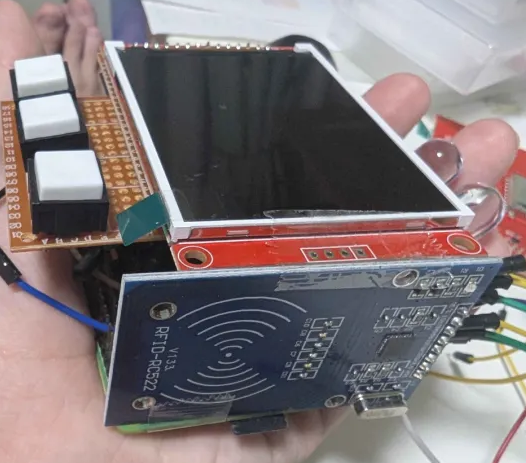
\includegraphics[width=\linewidth]{module.png}};
      \begin{scope}[x={(img.south east)}, y={(img.north west)},
          lbl/.style={fill=navy, text=white, rounded corners=5pt, inner sep=6pt,
            font=\fontsize{21pt}{24pt}\selectfont\bfseries},
          pt/.style={-{Circle[length=12pt]}, line width=3.5pt, color=navy}]
        \node[lbl] (l1) at (0.17,0.95) {ボタン};
        \draw[pt] (l1.south) -- (0.12,0.80);
        \node[lbl] (l2) at (0.62,0.92) {液晶};
        \draw[pt] (l2.south) -- (0.58,0.72);
        \node[lbl] (l3) at (0.30,0.10) {NFC};
        \draw[pt] (l3.north) -- (0.38,0.30);
      \end{scope}
    \end{tikzpicture}\\[4pt]
    \capt{試作したモジュール}
  \end{minipage}\hfill
  \begin{minipage}[t]{0.26\linewidth}\vspace{0pt}
    \centering
    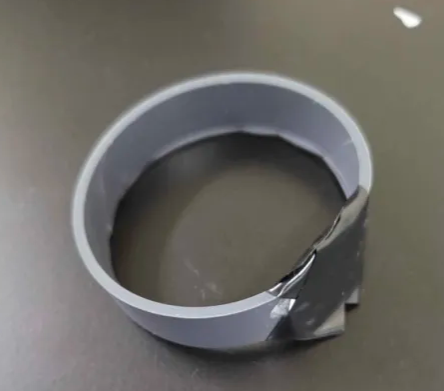
\includegraphics[width=0.92\linewidth]{watchdevice.png}\\[4pt]
    \capt{腕輪型タグ\\（社員証の代わり）\\手がふさがっても\\かざせる}
  \end{minipage}\hfill
  \begin{minipage}[t]{0.33\linewidth}\vspace{0pt}
    {\fontsize{24pt}{29pt}\selectfont
    \renewcommand{\arraystretch}{1.3}
    \begin{tabular}{@{}>{\bfseries\color{navy}}l@{\hspace{12pt}}l@{}}
      端末 & Raspberry Pi 4 \\
      読取 & NFC (RC522) \\
      表示 & 2.8 型液晶 \\
      入力 & ボタン 3 個 \\
      状態 & LED（赤＝作業中） \\
      通信 & MQTT \\
      AI   & Python \\
      音声 & Whisper \\
      LLM  & Gemma 3 \\
    \end{tabular}\par}
  \end{minipage}
  \vspace{14pt}
  \head{止まらない・迷わない工夫}
  {\centering
  \begin{tikzpicture}[font=\fontsize{21pt}{25pt}\selectfont]
    \tikzset{k/.style={draw=none, fill=card, rounded corners=8pt, text width=12.6cm,
      minimum height=2.4cm, align=left, inner sep=9pt}}
    \newcommand{\kk}[2]{{\bfseries\color{navy}\fontsize{24pt}{28pt}\selectfont #1}\\[3pt]{\color{ink2}#2}}
    \node[k] (k1) {\kk{サーバを自動で見つける}{モジュールは電源を入れるだけ}};
    \node[k, right=5mm of k1] (k2) {\kk{通信切れをすぐ表示}{MQTT の Last Will で管理画面へ}};
    \node[k, below=5mm of k1] (k3) {\kk{再起動しても復元}{作業中の状態をそのまま戻す}};
    \node[k, right=5mm of k3] (k4) {\kk{かざして登録}{新しいタグや機材を画面で紐付け}};
  \end{tikzpicture}\par}
}

% ================================================================ 右列
\column{0.5}

\block{\bt{現場での使い方}}{%
  \newcommand{\step}[3]{% 番号, 画面, 1 行
    \begin{minipage}[t]{0.238\linewidth}\vspace{0pt}\centering
      {\color{blue}\bfseries\fontsize{38pt}{38pt}\selectfont #1}\\[8pt]
      \photo{#2}{\linewidth}{0.75\linewidth}{}\\[8pt]
      {\fontsize{25pt}{31pt}\selectfont\bfseries #3\par}
    \end{minipage}}
  \step{1}{step1_menu.png}{腕輪をかざす}\hfill
  \step{2}{step2_task.png}{AI の提案を承認}\hfill
  \step{3}{step3_guide.png}{急ぐ仕事へ誘導}\hfill
  \step{4}{step4_done.png}{かざして完了}\par
  \vspace{8pt}
  \capt{モジュールの実際の画面（テストモードの仮想モジュールで撮影）}
  \vspace{16pt}

  \head{機材の状態の移り変わり}
  {\centering
  \begin{tikzpicture}[font=\fontsize{22pt}{26pt}\selectfont]
    \tikzset{c/.style={text width=4.2cm, minimum height=2.5cm, inner sep=6pt},
      e/.style={text width=6.0cm, inner sep=6pt}}
    \node[box, c, draw=blue, fill=skytint] (s1) {{\bfseries\color{blue} 空き}\\{\sm\color{ink2}LED 青}};
    \node[box, c, right=22mm of s1] (s2) {{\bfseries 仕事を提案}\\{\sm\color{ink2}1 件ずつ表示}};
    \node[obox, c, right=22mm of s2] (s3) {{\bfseries\color{orange} 作業中}\\{\sm\color{ink2}LED 赤}};
    \node[box, c, right=22mm of s3] (s4) {{\bfseries 完了を記録}\\{\sm\color{ink2}時間と体感}};
    \draw[arr] (s1) -- node[above=2pt, slab]{かざす} (s2);
    \draw[arr] (s2) -- node[above=2pt, slab]{承認} (s3);
    \draw[arr] (s3) -- node[above=2pt, slab]{かざす} (s4);
    \draw[arr, rounded corners=12pt] (s4.south) -- ++(0,-0.9) -| node[pos=0.25, below=2pt, elab]{機材を解放} (s1.south);
    % 例外
    \node[ybox, e, above=12mm of s2] (g) {{\bfseries 別の機材へ誘導}\\{\sm\color{ink2}本人宛の急ぎあり}};
    \draw[arr, color=yellowdeep] (s2) -- (g);
    \node[box, e, draw=ink2, above=12mm of s3] (f) {{\bfseries フリー利用}\\{\sm\color{ink2}提案を全部断った}};
    \draw[arr, color=ink2] (s2.north east) -- (f.south west);
    \draw[arr, color=ink2] (f) -- (s3);
    \node[box, e, draw=ink2, above=12mm of s4] (r) {{\bfseries 他の人は拒否}\\{\sm\color{ink2}取り合いなし}};
    \draw[arr, color=ink2, dashed] (s3.north east) -- (r.south west);
  \end{tikzpicture}\par}
  \vspace{12pt}
  \begin{minipage}[t]{0.31\linewidth}\vspace{0pt}\centering
    \photo{uc1_working.png}{\linewidth}{0.64\linewidth}{}\\[4pt]
    \capt{作業中：終わったら\\もう一度かざす}
  \end{minipage}\hfill
  \begin{minipage}[t]{0.31\linewidth}\vspace{0pt}\centering
    \photo{uc2_coming.png}{\linewidth}{0.64\linewidth}{}\\[4pt]
    \capt{誘導先の機材にも\\「向かっています」}
  \end{minipage}\hfill
  \begin{minipage}[t]{0.345\linewidth}\vspace{0pt}
    \begin{itemize}\fontsize{22pt}{28pt}\selectfont
      \item 終わったら体感を\\3 段階で答える\\→ \hl{AI の学習に使う}
      \item 操作はかざす・\\ボタンだけ\\→ \hl{PC が苦手でも安心}
    \end{itemize}
  \end{minipage}
}

\block{\bt{管理画面}}{%
  \begin{minipage}[c]{0.60\linewidth}
    \shot{0.97\linewidth}{admin_dashboard.png}\\[4pt]
    \capt{ダッシュボード：機材の使用中・空き}
  \end{minipage}\hfill
  \begin{minipage}[c]{0.38\linewidth}
    {\fontsize{22pt}{27pt}\selectfont
    \newcommand{\scr}[2]{{\bfseries\color{navy}#1}\par{\color{ink2}#2}\par\vspace{8pt}}
    \scr{ダッシュボード}{稼働状況を自動で更新}
    \scr{タスク管理}{重要度・期限・資格を登録\\「AI 割当」ボタン}
    \scr{作業者管理}{経験年数・資格・タグ}
    \scr{機材管理}{紐付け・通信状態}
    \vspace{2pt}
    {\bfseries ブラウザだけで完結}\par}
  \end{minipage}
}

\block{\bt{使う人のメリット}}{%
  \newcommand{\mt}[2]{{\bfseries\fontsize{25pt}{30pt}\selectfont #1\par}{\fontsize{20pt}{24pt}\selectfont\color{ink2}#2\par}\vspace{9pt}}
  \begin{minipage}[t]{0.488\linewidth}\vspace{0pt}
    \tint{goodtint}{%
      {\centering{\fontsize{32pt}{38pt}\selectfont\bfseries\color{good}従業員}\par}
      \vspace{10pt}
      \mt{腕輪をかざすだけ}{PC・スマホの操作もなし}
      \mt{仕事を探さなくてよい}{かざすと次の仕事が出る}
      \mt{完了報告がいらない}{時間は自動で記録}
      \mt{機材の取り合いがない}{使用中は画面に表示}
      \mt{新人にもチャンス}{AI が試しに任せる}
      \mt{声で仕事を登録}{ボタンを押して話すだけ}}
  \end{minipage}\hfill
  \begin{minipage}[t]{0.488\linewidth}\vspace{0pt}
    \tint{skytint}{%
      {\centering{\fontsize{32pt}{38pt}\selectfont\bfseries\color{blue}管理者}\par}
      \vspace{10pt}
      \mt{現場が一目で分かる}{誰が・どこで・何を}
      \mt{割り振りは AI}{ボタン 1 つで担当者決定}
      \mt{得意・不得意が分かる}{作業ログから自動で収集}
      \mt{仕事の偏りを防ぐ}{手持ちの多い人を避ける}
      \mt{安全を守る}{無資格者に危険作業なし}
      \mt{IT 担当者が不要}{ブラウザだけで管理、運営}}
  \end{minipage}
}

\end{columns}

\end{document}
